Robotic manipulation, where a robot \textit{physically} interacts and changes the environment, is one of the most challenging tasks in robot autonomy from the perspectives of perception, planning, and control. Consider a simple pick-and-place problem: the robot needs to identify the object, find a good place to grasp, stably pick up the object, and move it to a new location, all while ensuring no part of the robot collides with the environment. In practice even this simple task can become much harder, for example if other objects are in the way and must be moved first, if the object does not have particularly good grasping features, if the weight, size, and surface texture of the object is unknown, or if the lighting is poor\footnote{Generally speaking the infinite variability of the real world makes \textit{robust} manipulation extremely difficult.}. Manipulation tasks are also commonly composed of sequences of interactions, such as making a sandwich or opening a locked door. This chapter focuses on \textit{grasping}\cite{PrattichizzoTrinkle2016}, which is a fundamental component to all manipulation tasks.

\notessection{Grasping}
Grasping is a fundamental component of robotic manipulation that focuses on obtaining complete control of an object's motion (in contrast to other interactions such as pushing). 
\begin{definition}[Grasp]
A \textit{grasp} is an act of restraining an object's motion through application of forces and torques at a set of contact points.
\end{definition}
\begin{marginfigure} 
\begin{center}
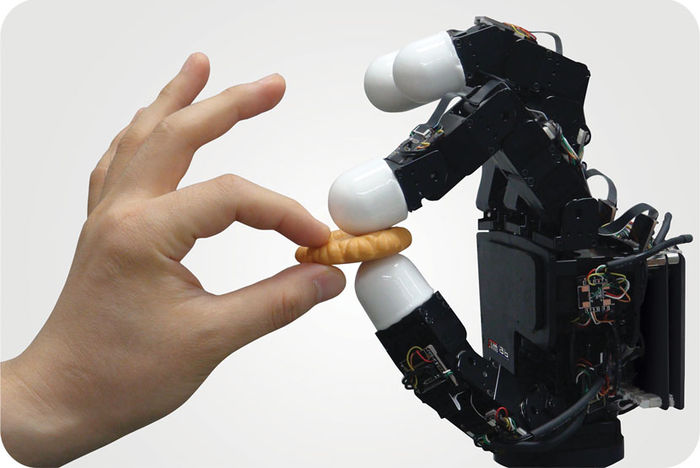
\includegraphics[width=0.95\textwidth]{tex/figs/ch26_figs/allegrohand.jpg}
\caption{The Allegro Hand. Image retrieved from \texttt{wiki.wonikrobotics.com}.}
\label{fig:allegrohand}
\end{center}
\end{marginfigure}
Grasping is challenging for several reasons:
\begin{enumerate}
    \item The configuration of the gripper may be high-dimensional. For example the Allegro Hand (Figure \ref{fig:allegrohand}) has 4 fingers with 3 joints each for a total of 12 dimensions. Plus there are an additional 6 degrees of freedom in the wrist posture (position and orientation), and all of these degrees of freedom vary continuously.
    \item Choosing contact points can be difficult. An ideal choice of contact points would lead to a robust grasp, but the space of feasible contacts is restricted by the gripper's geometry. A rigid body object also has 6 degrees freedom, which affects where the contact points are located in the robot's workspace.
    \item While the robot is attempting the grasp it must be sure that its entire body does not come into collision with the environment.
    \item Once a grasp has been performed it is important to evaluate how robust the grasp is. While the grasp quality would ideally be optimized during the planning step, it may be important to also check retroactively in case uncertainty led to a different grasp than planned.
\end{enumerate}

To address each of these challenges, the grasp can be subdivided into parts: planning, acquisition/maintenance, and evaluation. This chapter will focus on the fundamentals of how a grasp can be \textit{modeled} and \textit{evaluated} from a mathematical perspective, as well as how grasps can be \textit{planned}\footnote{Part of grasp planning also includes the motion planning of the entire robot, but the focus of this chapter is on the grasp itself.} using grasp force optimization. Learning-based approaches to grasping and manipulations will also be discussed at a high level in Section \ref{subsec:grasplearning} and \ref{subsec:manipulationlearning}.

\subsection{Grasp Modeling} \label{subsec:graspmodel}
A grasp plan may be parameterized in several ways, including by the approach vector or wrist orientation of the gripper, by the initial finger configuration, or directly by points of contact with the object. However, regardless of the planning parameterization the resulting contacts between the gripper and the object will define the quality of the grasp. Therefore it is useful and convenient for grasp modeling to consider the contact points as the interaction interface between the gripper and object.

\subsubsection{Contact Types}
There are generally three types of contact that can occur in grasping scenarios:
\begin{enumerate}
    \item \textit{Point}: a point contact occurs when a single point comes in contact with either another point, a line, or a plane. A point contact is only stable if it is a point-on-plane contact\footnote{Point-on-plane contacts are by far the most commonly modeled contact types and will almost always be used in grasp analysis.}, point-on-point or point-on-line contacts are unstable.
    \item \textit{Line}: line contacts occur when a line comes in contact with another line or a plane. Line-on-plane and line-on-nonparallel line contacts are stable, but line-on-parallel line contacts are unstable. Line contacts can also be represented as two point contacts.
    \item \textit{Plane}: plane-on-plane contacts are always stable. Plane contacts can also be represented as point contacts by converting a distribution of normal forces across a region into a weighted sum of point forces at the vertices of the region's convex hull.
\end{enumerate}
\begin{figure}[ht]
\begin{center}
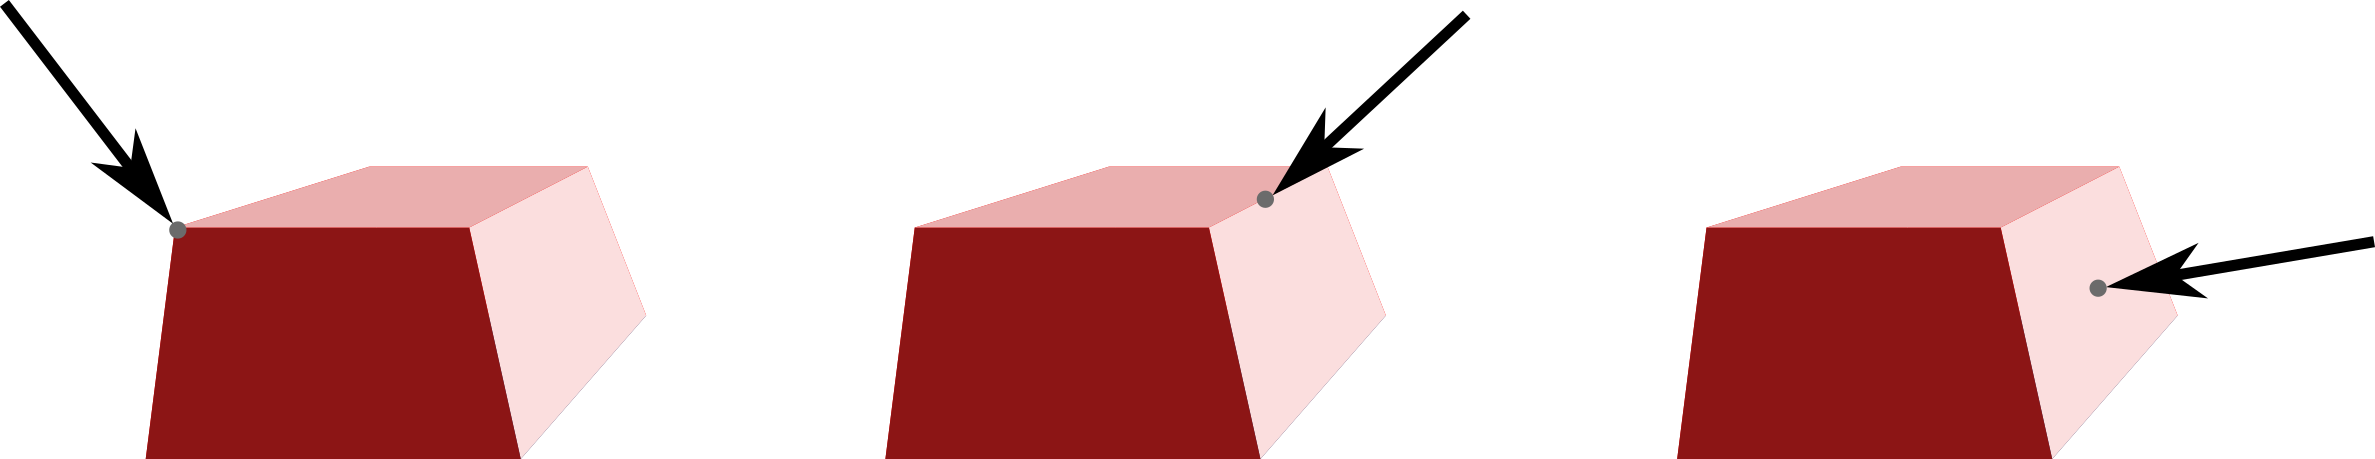
\includegraphics[width=0.9\textwidth]{tex/figs/ch26_figs/contacts.png}
\caption{Grasping contacts are generally either point-on-point (left), point-on-line (middle), point-on-plane (right).}
\label{fig:contacts}
\end{center}
\end{figure}

\subsubsection{Point-on-Plane Contact Models}
Point-on-plane contact models are by far the most commonly used for grasping since the possible contact points for most objects are almost always surface points (and not sharp edges or points).
The purpose of the contact model is to specify the admissible forces and torques that can be transmitted through a particular contact. Considering a local reference frame defined at the contact point with the $z$ direction pointing along the object's surface normal (with the positive direction defined as into the object), the force $\f$ can be written as:
\begin{equation*}
        \f = \f_{\text{normal}} + \f_{\text{tangent}},
\end{equation*}
where $\f_{\text{normal}} = [0,\: 0,\: f_z ]^\top $ is the vector component along the normal direction (with magnitude $f_z$) and $\f_{\text{tangent}} =[f_x,\: f_y,\: 0 ]^\top $ is the vector component tangent to the surface. For all types of contact only an inward force can be applied, therefore $f_z \geq 0$. Three types of contact models are commonly used, and each defines a set $\mathcal{F}$ of admissible forces that can be applied through the contact:
\begin{enumerate}
    \item Frictionless Point Contact: forces can only be applied along the surface normal, no torques or forces tangential with the surface are possible ($\f_{\text{tangent}} = 0$):
    \begin{equation*}
        \mathcal{F} = \{\f_{\text{normal}} \mid f_z \geq 0\}.
    \end{equation*}
    These types of contact models are more common in form closure grasps.
    
    \item Point Contact with Friction\footnote[][-8\baselineskip]{Also referred to as the \textit{hard finger} model.}: it is possible to apply forces in directions other than just the surface normal. The admissible forces (i.e. forces that don't lead to slipping) are typically defined by a \textit{friction cone}:
    \begin{equation*}
        \mathcal{F} = \{\f \mid \lVert \f_{\text{tangent}} \rVert \leq \mu_s\lVert  \f_{\text{normal}}  \rVert, \quad f_z \geq 0\}.
    \end{equation*}
    where $\mu_s$ is the static friction coefficient associated with the surface (see Figure \ref{fig:frictioncone}).
    \begin{marginfigure}[-15\baselineskip] 
    \begin{center}
    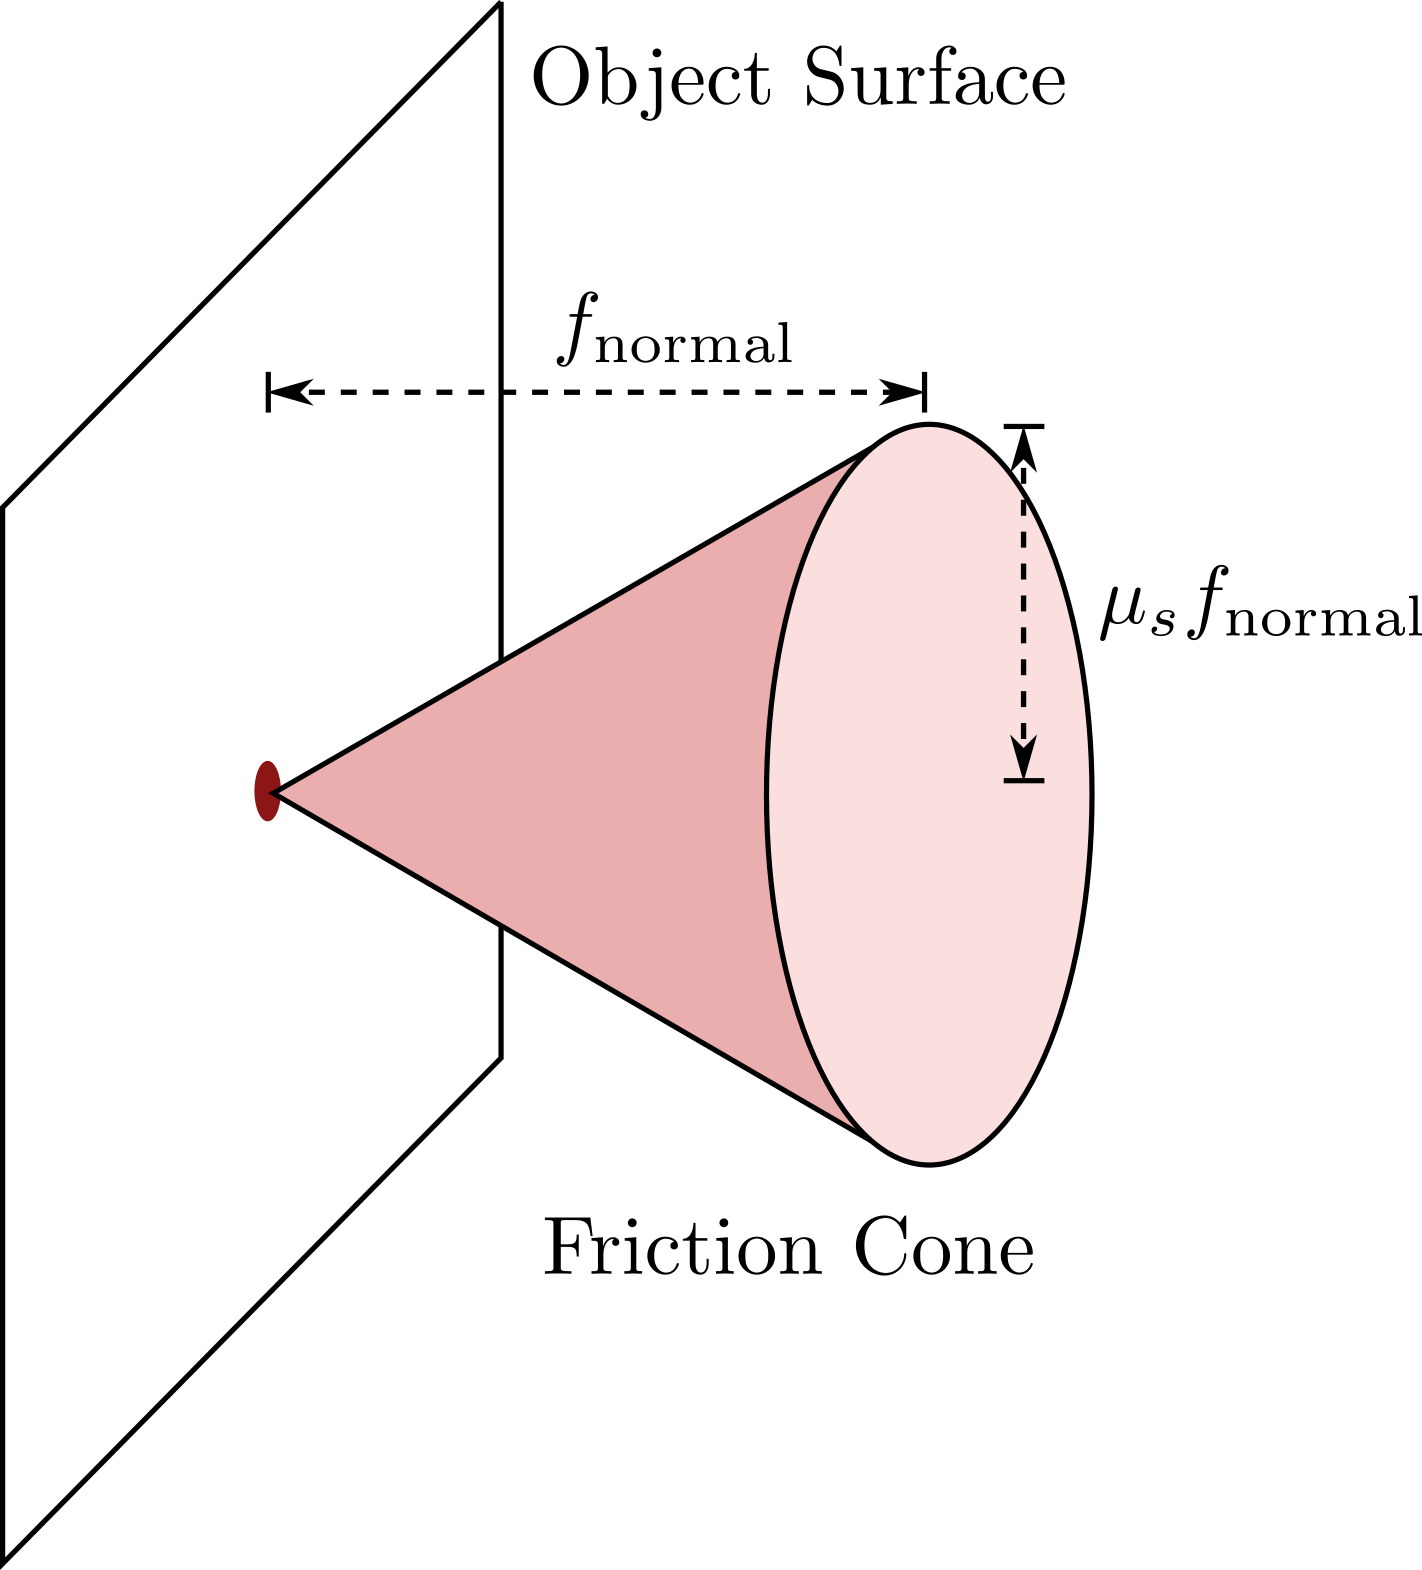
\includegraphics[width=0.95\textwidth]{tex/figs/ch26_figs/frictioncone.png}
    \caption{Friction cone defined by a static coefficient of friction $\mu_s$.}
    \label{fig:frictioncone}
    \end{center}
    \end{marginfigure}
    \begin{marginfigure} 
    \begin{center}
    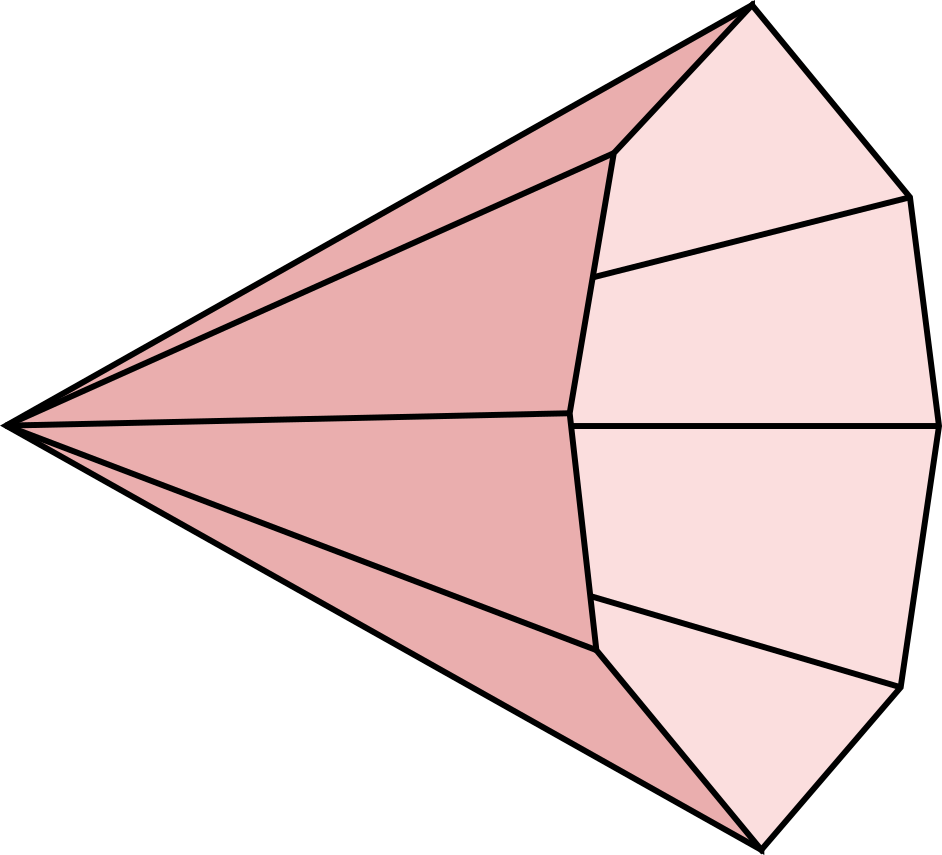
\includegraphics[width=0.55\textwidth]{tex/figs/ch26_figs/linearfrictioncone.png}
    \caption{Linearized friction cone to \textit{inner} approximate the true cone.}
    \label{fig:linearcone}
    \end{center}
    \end{marginfigure}
    A pyramidal inner-approximation of the friction cone is often more useful from a computational standpoint, since its definition only requires a \textit{finite} set of vectors (see Figure \ref{fig:linearcone}).
    The point contact with friction model is more common in force closure grasps.
    \item Soft-finger Contact Model: allows for a torque $\tau_{\text{normal}}$ around the surface normal axis and also includes a friction cone for the forces as in the point contact with friction model. The admissible torques are also constrained by friction:
    \begin{equation*}
        \mathcal{F} = \{(\f, \tau_{\text{normal}}) \mid \lVert \f_{\text{tangent}} \rVert \leq \mu_s\lVert  \f_{\text{normal}}  \rVert, \quad f_z \geq 0, \quad \lvert \tau_{\text{normal}} \rvert \leq \gamma f_z\}.
    \end{equation*}
    where $\gamma > 0$ is the torsional friction coefficient.
\end{enumerate}

\subsubsection{Wrenches and Grasp Wrench Space}
Under the assumption of a specific contact model, a grasp (defined by a set of contact points) can be quantified and evaluated by determining the \textit{grasp wrench space}\footnote{The grasp wrench space is a \textit{subset} of the \textit{wrench space} $\R^n$, where $n = 6$ in 3D settings and $n=3$ in 2D settings.}, which defines how the grasp can influence the object through an applied wrench.
\begin{definition}[Wrench]
A \textit{wrench} is a vector valued quantity that describes the forces and torques being applied to an object. For a force $\f \in \R^3$ and torque $\btau \in \R^3$ applied at the object's center of mass, the wrench is the stacked vector: 
\begin{equation*}
    \w = \begin{bmatrix}
    \f \\ \btau
    \end{bmatrix} \in \R^6,
\end{equation*}
and is typically written with respect to a frame fixed in the body. 
\end{definition}
Each contact point $i$ in a grasp applies a wrench to the object. Additionally the torque $\btau_i$ can be computed by $\btau_i = \bd_i \times \f_i$ where $\bd_i$ is the vector defining the position of the $i$-th contact point with respect to the object's center of mass.
The wrench can then be written as:
\begin{equation} \label{eq:contactwrench}
    \w_i = \begin{bmatrix}
    \f_i \\ \lambda(\bd_i \times \f_i)
    \end{bmatrix},
\end{equation}
where the constant $\lambda \in \R$ is arbitrary but can be used to scale the torque magnitude if desired\footnote[][-4\baselineskip]{If the forces $\f_{i,j}$ are dimensional a value of $\lambda=1$ is common. When the forces are unit-dimension (i.e. scaled by their maximum magnitude), $\lambda$ could be chosen to non-dimensionalize the entire wrench $\w_i$ by non-dimensionalizing the distance vector $\bd_i$ (i.e. scale by an object size metric).}. 

Using this definition of a wrench\footnote[][2\baselineskip]{For a soft-finger contact model the additional torque term must also be included.}, a grasp can be defined as the set of all possible wrenches that can be achieved by the grasp's contact points. Mathematically, an admissible force $\f_i$ applied at the $i$-th contact point can be linearly mapped into the corresponding wrench on the object as $G_i\f_i$, where $G_i$ is a wrench basis matrix that also includes a transformation from the local contact reference frame to an object-defined global reference frame. Therefore the total wrench on the object from all contacts is:
\begin{equation} \label{eq:graspmap}
    \w = \sum_{i=1}^k G_i \f_i = G\begin{bmatrix} 
    \f_1 \\ \vdots \\ \f_k
    \end{bmatrix}, \quad G = \begin{bmatrix} 
    G_1 & \dots & G_k
    \end{bmatrix},
\end{equation}
where the combined matrix $G$ is referred to as the \textit{grasp map} (which varies depending on the type of contact model used).

The \textit{grasp wrench space} can then be defined as:
\begin{definition}[Grasp Wrench Space]
The grasp wrench space $\mathcal{W}$ for a grasp with $k$ contact points is the set of all possible wrenches $\w$ that can be applied to the object through admissible forces:
\begin{equation} \label{eq:graspwrenchspace}
\mathcal{W} \coloneqq \{\w \mid \w = \sum_{i=1}^k G_i \f_i, \quad \f_i \in \mathcal{F}_i, \quad i = 1,\dots,k\}.
\end{equation}
\end{definition}
In other words, the grasp wrench space is defined by the output of \eqref{eq:graspmap} over all possible applied force combinations $\{\f_i\}_{i=1}^k$.
If the grasp wrench space is large the grasp can compensate for a bigger set of external wrenches that might be applied to the object, leading to a more robust grasp.

\begin{example}[Computing a Grasp Wrench Space from Friction Cones] \label{ex:2Dgrasp}
Consider a grasping problem with $k$ contact points with friction, and let contact point $i$ be associated with a linearized friction cone $\mathcal{F}_i$ whose edges are defined by the set of $m$ forces:
\begin{equation*}
    \{\f_{i,1}, \f_{i,2}, \dots \f_{i,m}\},
\end{equation*}
such that any force $\f_i \in \mathcal{F}_i$ can be written as a positive combination of these vectors:
\begin{equation*}
    \f_i = \sum_{j=1}^m \alpha_{i,j}\f_{i,j}, \quad \alpha_{i,j} \geq 0.
\end{equation*}
The condition $\sum_{j=1}^m \alpha_{i,j} \leq 1$ will also be imposed to constrain the overall magnitude\footnote[][]{In practice the physical hardware has limitations on the magnitude of the normal forces that can be applied.}. Geometrically, this means that the friction cone $\mathcal{F}_i$ is the convex hull of the points $\f_{i,j}$ and the origin of the local contact reference frame (see Figure \ref{fig:linearcone2}).
\begin{marginfigure} 
\begin{center}
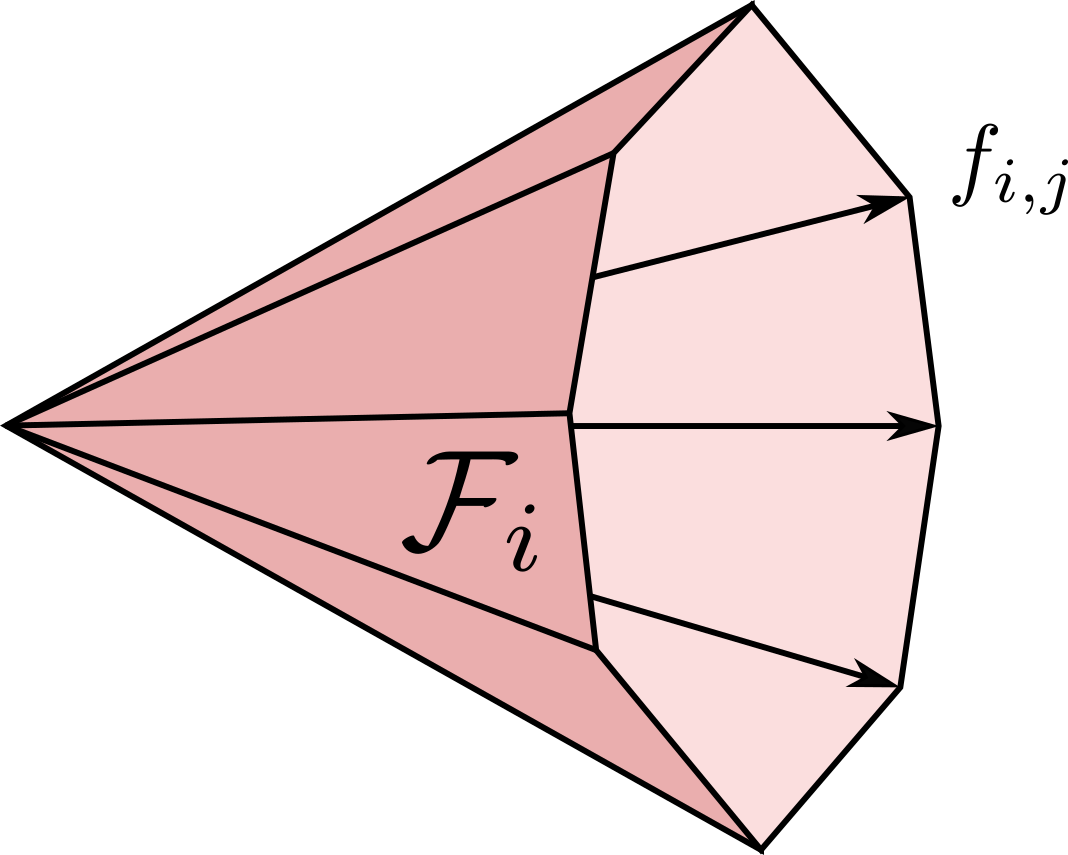
\includegraphics[width=0.65\textwidth]{tex/figs/ch26_figs/linearfrictioncone2.png}
\caption{Any force $\f_i \in \mathcal{F}_i$ can be written as a convex combination of the forces along the edge vectors $\f_{i,j}$.}
\label{fig:linearcone2}
\end{center}
\end{marginfigure}

This friction cone can then be mapped into the wrench space using \eqref{eq:contactwrench}. Assuming the forces $\f_{i,j}$ and position vector $\bd_i$ are already expressed in a reference frame fixed in the object that is common to all $i$ contact points, the grasp wrench space $\mathcal{W}$ can be written as:
\begin{equation*}
\begin{split}
\mathcal{W} = \{\w \mid \w = \sum_{i=1}^k \w_i, \quad &\w_i = \sum_{j=1}^m \alpha_{i,j}\w_{i,j}, \quad \w_{i,j} = \begin{bmatrix}
    \f_{i,j} \\ \lambda(\bd_i \times \f_{i,j})
    \end{bmatrix}, \\
&\sum_{j=1}^m \alpha_{i,j} \leq 1, \quad \alpha_{i,j} \geq 0\}.    
\end{split}
\end{equation*}
In other words, the grasp wrench space is defined by taking the Minkowski sum over the sets of wrenches that can be generated from each individual contact!

\begin{figure}[ht]
\begin{center}
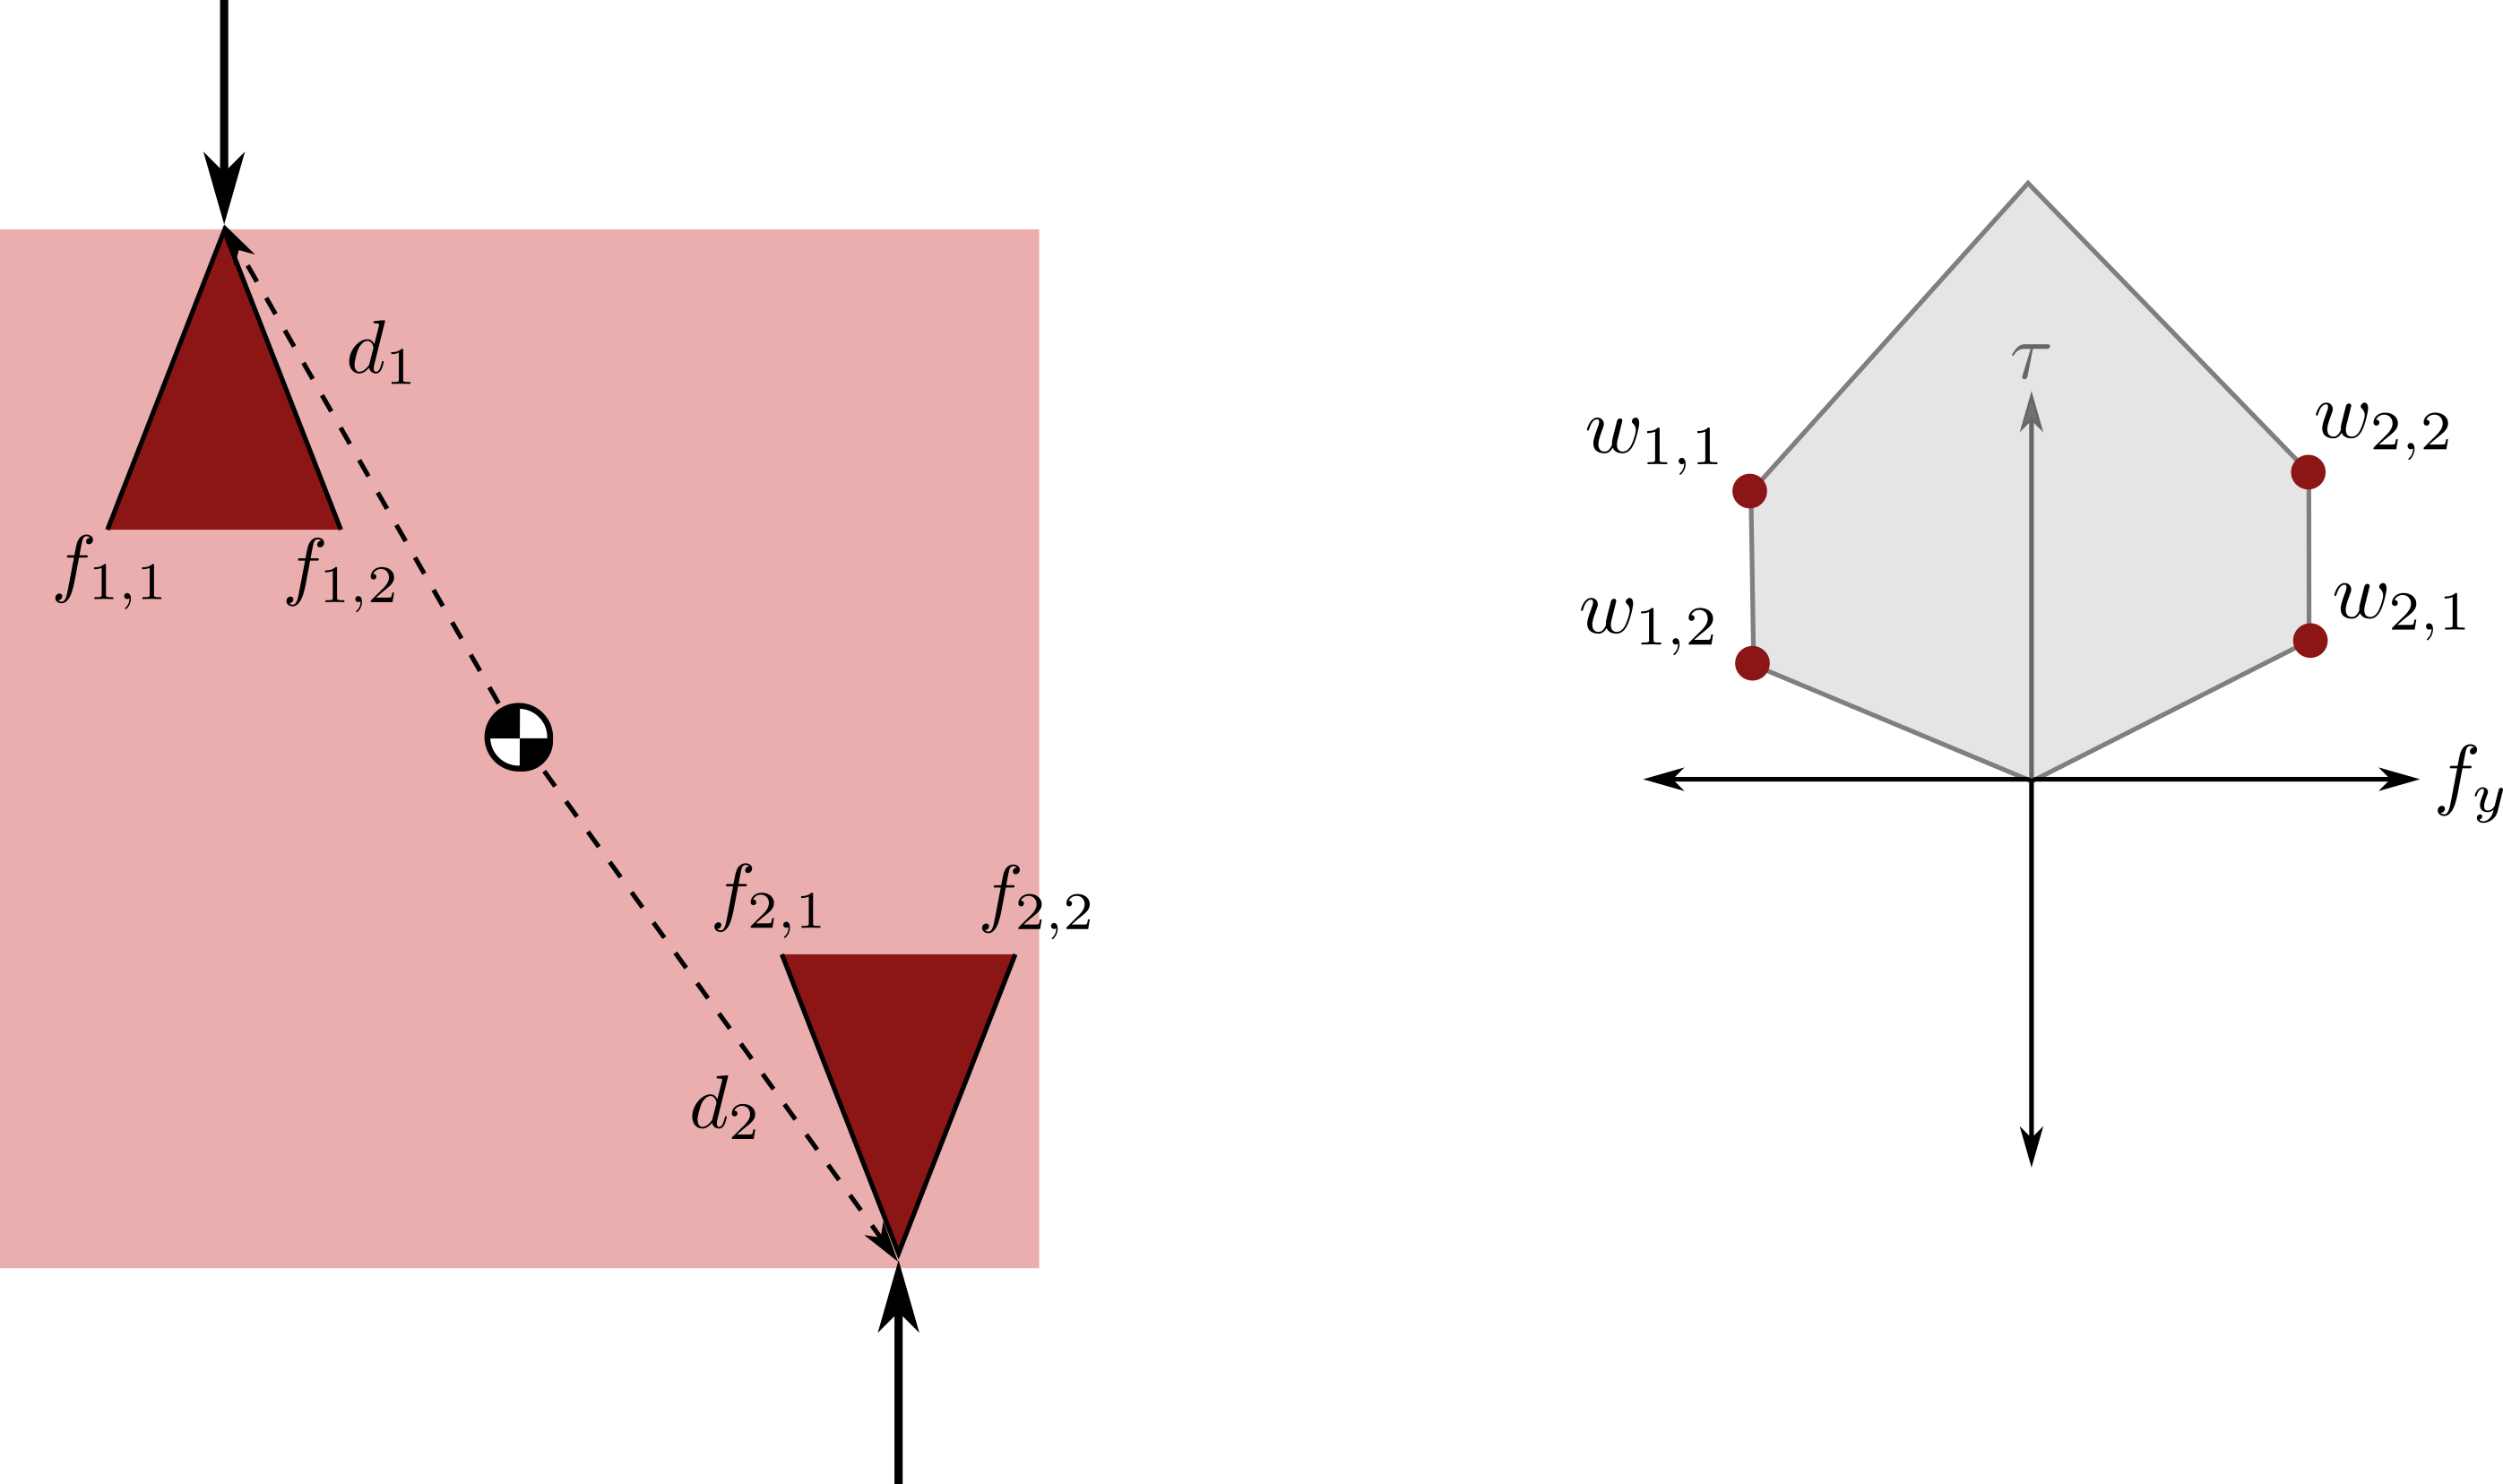
\includegraphics[width=0.75\textwidth]{tex/figs/ch26_figs/2Dexample_a.png}
\caption{An example 2D grasp consisting of two point contacts with friction. The friction cones shown in the figure on the left yield the grasp wrench space in the figure on the right (showing only the vertical force and torque dimensions). Note that the grasp wrench space is bounded because it is assumed the magnitude of the contact forces are bounded. The solid grey line represents the boundary of $\mathcal{W}$.}
\label{fig:2dgrasp_a}
\end{center}
\end{figure}
For example, consider the 2D problem shown in Figure \ref{fig:2dgrasp_a} where there are $k=2$ contact points with friction. The friction cones are defined by the convex hull of the vectors $\{\f_{1,1},\f_{1,2}\}$ and $\{\f_{2,1},\f_{2,2}\}$ (and their origins) and the distance vectors from the center of mass to the contact points are $\bd_1$ and $\bd_2$. The force vectors $\f_{i,j}$ are then mapped into the wrenches $\w_{i,j}$ (shown on a 2D plot of vertical force $f_y$ and torque $\tau$ in Figure \ref{fig:2dgrasp_a}, ignoring the horizontal force components $f_x$). 
The grasp wrench space $\mathcal{W}$ is then shown in the grey region of the wrench space, where the solid grey line is the boundary of $\mathcal{W}$.
\end{example}

\subsection{Grasp Evaluation} \label{subsec:graspeval}
Now that the basics of grasp modeling have been introduced\footnote{contact types, contact models, grasp wrench spaces} it is possible to explore techniques for evaluating whether a grasp is ``good''. In particular, an ideal grasp is one that has \textit{closure}.
\begin{definition}[Grasp Closure]
Grasp closure occurs when the grasp can be maintained for every possible disturbance load.
\end{definition}
For example having grasp closure on a book would enable the gripper to maintain its grasp even if the book was hit by another object or if another book was suddenly stacked on top of it. In practice it may not be reasonable to assume that every \textit{magnitude} disturbance load could be accounted for, but the concept of closure is useful nonetheless.

It can also be helpful to distinguish between two types of grasp closure. A \textit{form closure}\footnote[][-5\baselineskip]{Also called power grasps or enveloping grasps. A grasp must have at least seven contacts to provide form closure for a 3D object.} grasp typically has the gripper joint angles locked and there is no ``wiggle'' room for the object (i.e. the object is kinematically constrained). Alternatively, a \textit{force closure}\footnote{Also called a precision grasp. Under a point contact with friction model, a grasp must have at least three contacts to provide force closure for a 3D object.} grasp uses forces applied at contact points to be able to \textit{resist} any external wrench. Force closure grasps typically rely on \textit{friction} and generally require fewer contact points than are required for form closure, but may not be able to actually cancel all disturbance wrenches if the friction forces are too weak. This chapter will primarily focus on evaluating force closure grasps since these are most common in robotics.
\begin{figure}[ht]
\begin{center}

\includegraphics[width=0.8\textwidth]{tex/figs/ch26_figs/closure.png}
\caption{Examples of grasps with form closure (left) and force closure under the soft-finger contact model (right).}
\label{fig:closure}
\end{center}
\end{figure}

\subsubsection{Force Closure Grasps}
The concept of force closure can be related to the grasp modeling concepts from Section \ref{subsec:graspmodel}:
\begin{definition}[Force Closure Grasp] \label{def:forceclosure}
A grasp is a \textit{force closure grasp} if for any external wrench $\w$ there exist contact forces $\{\f_i\}_{i=1}^k$ such that:
\begin{equation*}
-\w = \sum_{i=1}^k G_i \f_i. \quad \f_i \in \mathcal{F}_i, \quad i = 1, \dots, k,
\end{equation*}
or equivalently such that:
\begin{equation*}
    -\w \in \mathcal{W}.
\end{equation*}
\end{definition}
This definition implies that the grasp wrench space must satisfy $\mathcal{W} = \R^n$ for a force closure grasp, which implicitly assumes that the contact forces can be infinite in magnitude.\footnote{For 2D objects $n=3$ and for 3D objects $n=6$.} Since real hardware has limitations on the magnitude of the applied contact forces, a more practical definition of force closure is to be able to \textit{resist} any external wrenches.
The conditions for force closure can be summarized by the following theorem:
\begin{theorem}[] \label{thm:vectorclosure}
In an $n$-dimensional vector space with:
\begin{equation*}
\mathcal{W} \coloneqq \{\w \mid \w = \sum_{k=1}^{N} \beta_k \w_k, \quad \beta_k \geq 0\},
\end{equation*}
$\mathcal{W} = \R^n$ if and only if the set $\{\w_k\}_{k=1}^N$ contains at least $n+1$ vectors, $n$ of the vectors are linearly independent, and there exists scalars $\beta_k > 0$ such that:
\begin{equation*}
\sum_{k=1}^{N} \beta_k \w_k = 0.
\end{equation*}
\end{theorem}
From a practical perspective this theorem specifies a minimum number of different wrenches that must be used as a basis for the grasp wrench space, and also states that it must be possible for the grasp to apply zero wrench \textit{even when some of the contact forces are non-zero}. These conditions are equivalent to saying that grasp wrench space $\mathcal{W}$ must contain the origin in its \textit{interior}\footnote{The grasp is not in force closure if the origin is on the \textit{boundary} of $\mathcal{W}$.}. 

Note that in the practical case where the applied contact forces are assumed to be bounded, the conditions of Theorem \ref{thm:vectorclosure} must still hold to guarantee the origin is in the interior of $\mathcal{W}$, which is required to resist any external wrench.
The implications of this theorem are explored further in the following examples.

\begin{example}[2D Object (Forces Only)]
Consider a simplified 2D problem where instead of complete force closure (i.e. ability to withstand any \textit{wrench}) it is sufficient to only require the cancellation of external \textit{forces}. In this case $n=2$ and Theorem \ref{thm:vectorclosure} states that it must be possible for the grasp to generate $3$ force vectors where $2$ are linearly independent and where:
\begin{equation*}
\beta_1 \f_1 + \beta_2 \f_2 + \beta_3 \f_3 = 0, \quad \beta_1, \beta_2, \beta_3 > 0.
\end{equation*}
Two examples grasps are shown in Figures \ref{fig:2dgrasp_forces_a} and \ref{fig:2dgrasp_forces_b}. In Figure \ref{fig:2dgrasp_forces_a} the three contacts are frictionless, but even though there are 3 possible force vectors with 2 linearly independent, there is no way to generate zero force with non-zero forces at each contact! Therefore this grasp does not have force closure. 
\begin{figure}[ht]
\begin{center}
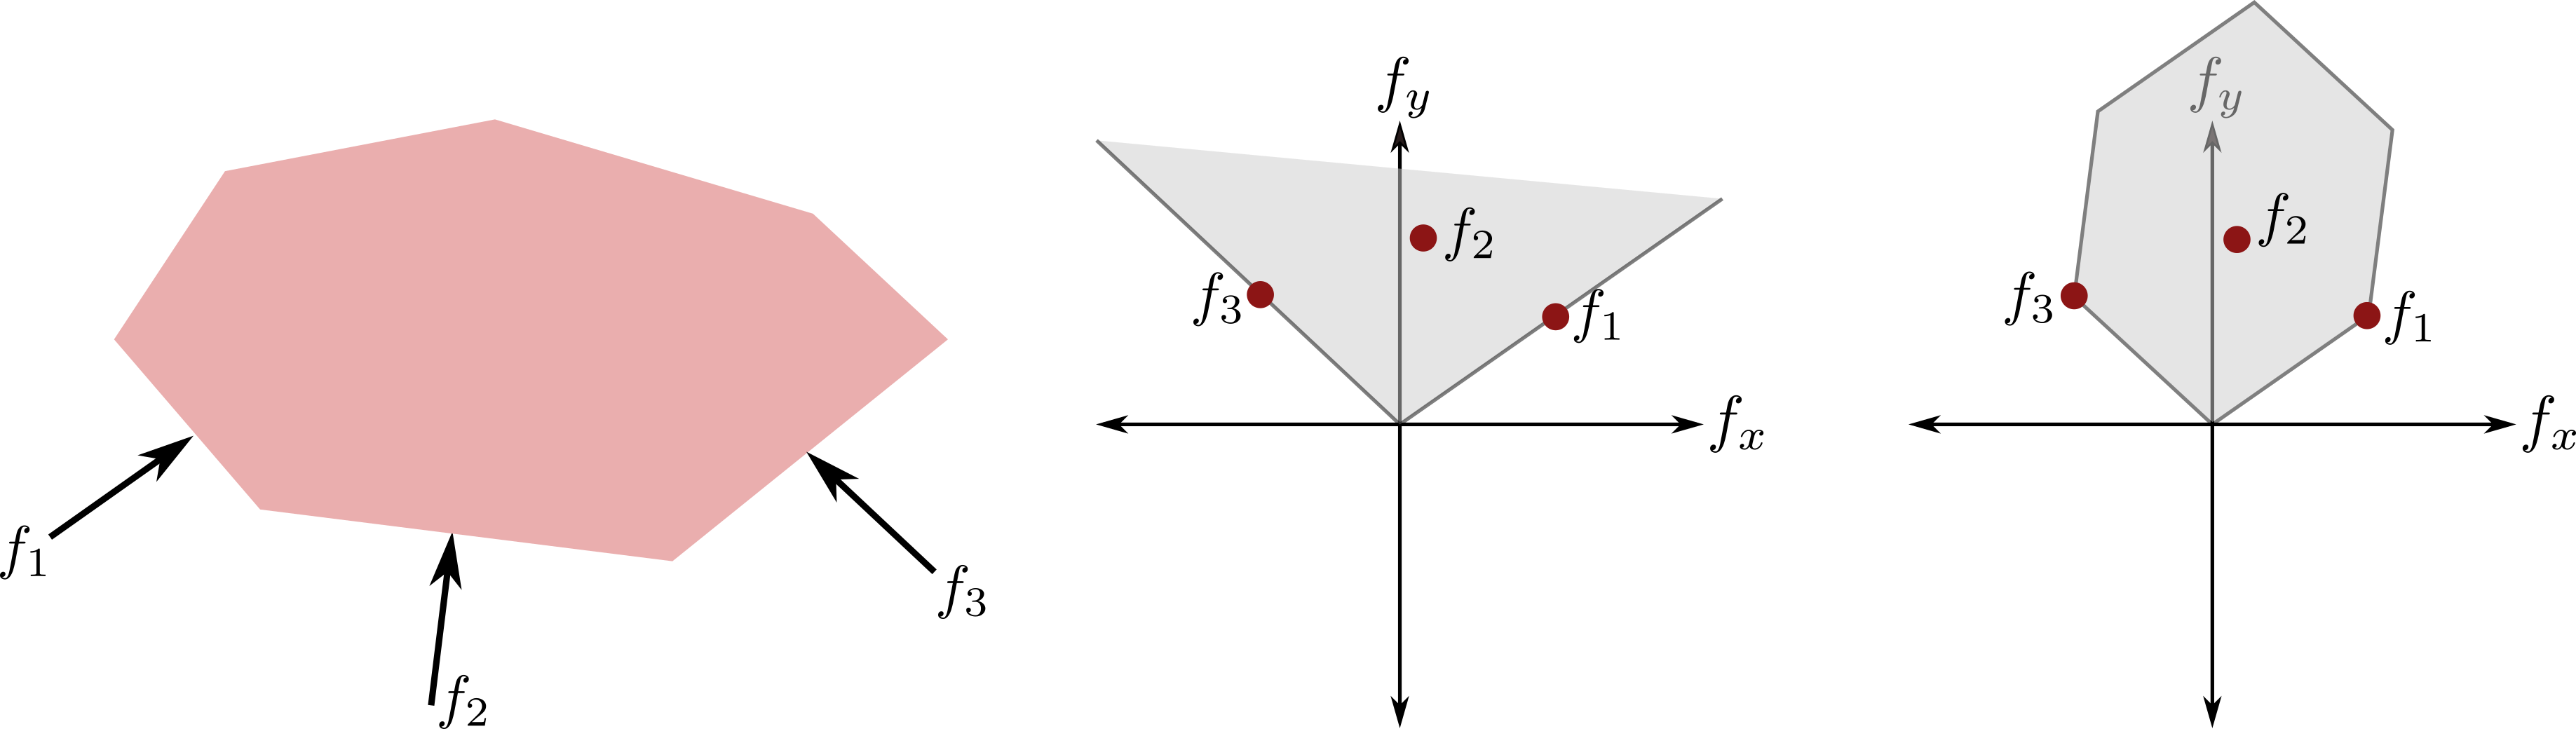
\includegraphics[width=0.9\textwidth]{tex/figs/ch26_figs/2Dexample_forces_a.png}
\caption{A 2D grasp with frictionless contacts that cannot compensate for all possible external forces on the object. The middle and right-side figures show the space of all possible applied forces for the cases of unbounded and bounded contact force magnitude, respectively.}
\label{fig:2dgrasp_forces_a}
\end{center}
\end{figure}

Alternatively, Figure \ref{fig:2dgrasp_forces_b} shows a case where it is possible to have force closure using a point contact without friction and a point contact with friction (a hypothetical example). In this case all of the conditions in Theorem \ref{thm:vectorclosure} are satisfied, and it can be seen that the origin is contained in the interior of the space of possible applied forces.
\begin{figure}[ht]
\begin{center}
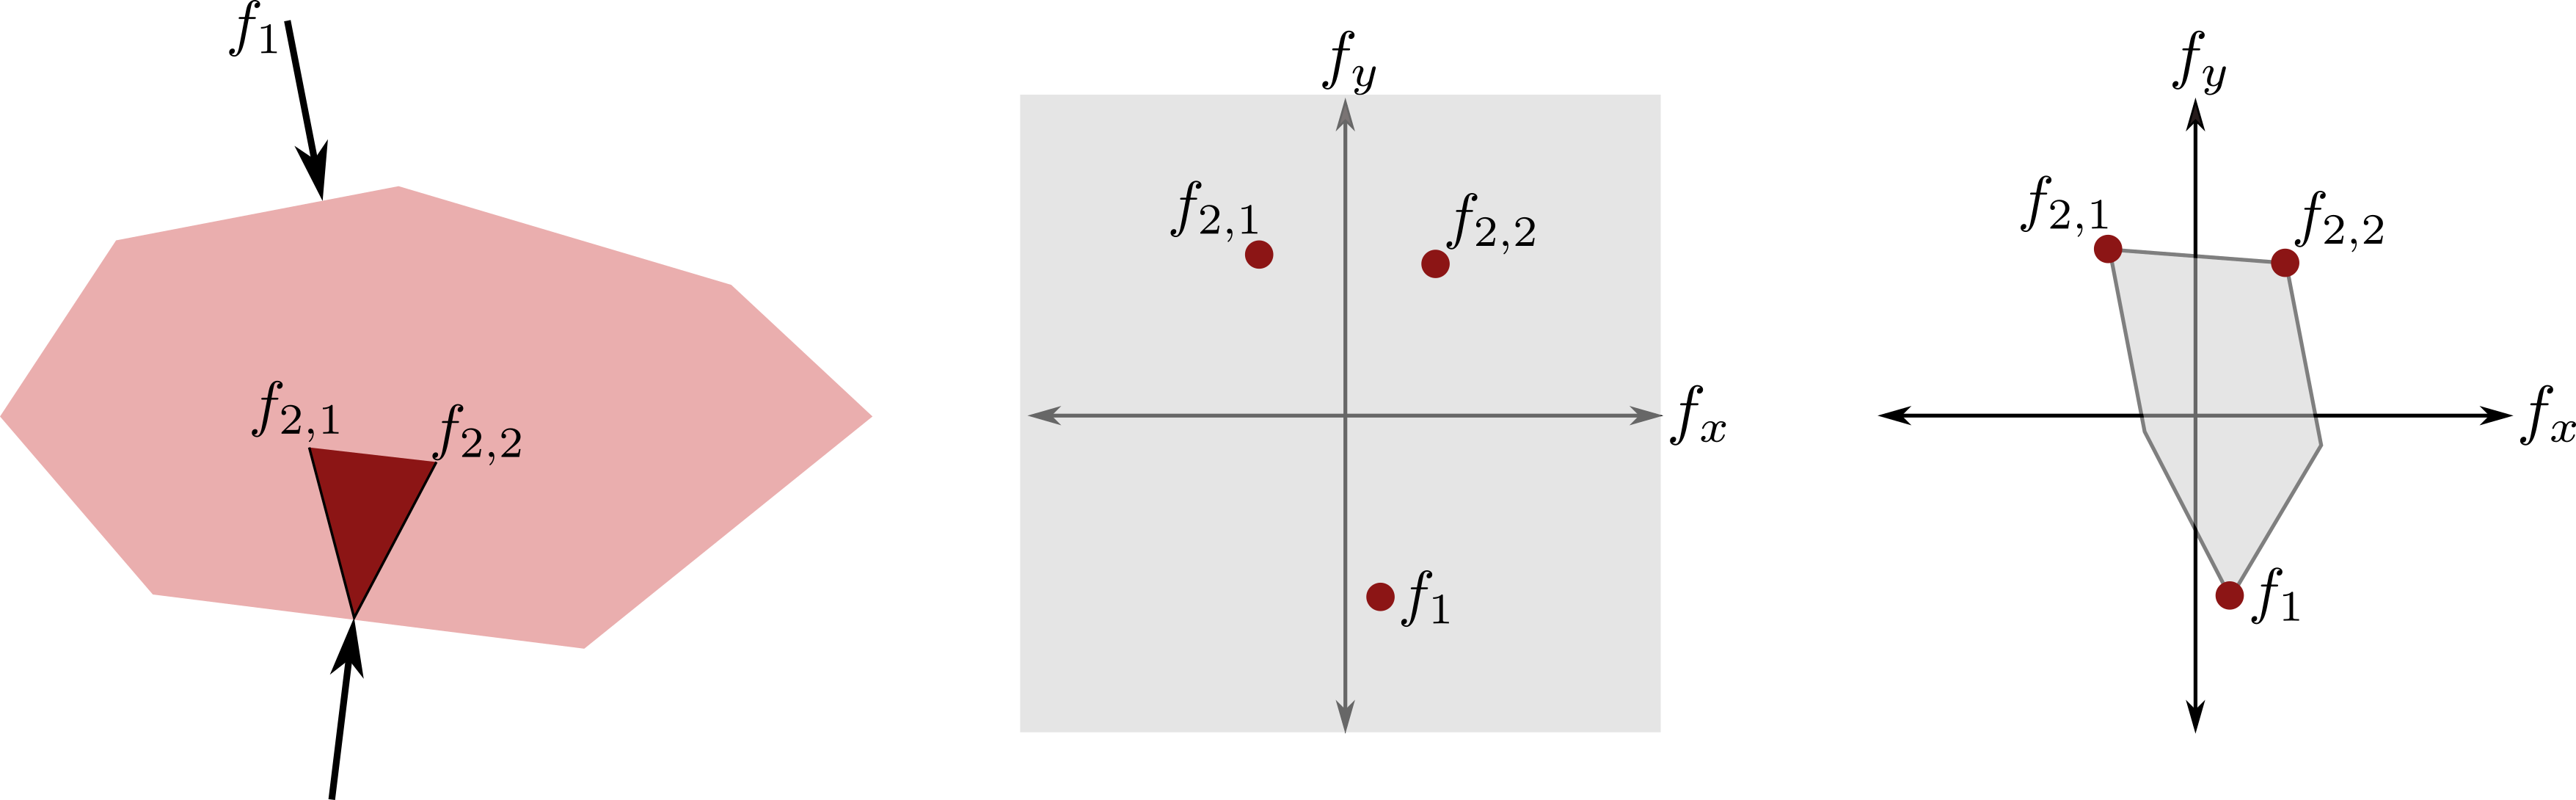
\includegraphics[width=0.9\textwidth]{tex/figs/ch26_figs/2Dexample_forces_b.png}
\caption{A 2D grasp consisting of a contact with friction and a contact without friction. The middle and right-side figures show the space of possible forces for the cases of unbounded and bounded magnitude, respectively. In the unbounded case it is possible to compensate for any external force, and in the bounded case it is possible to \textit{resist} an arbitrary force.}
\label{fig:2dgrasp_forces_b}
\end{center}
\end{figure}
\end{example}

\begin{example}[2D Object] \label{ex:2dobject}
In the more general case with 2D objects where the torque is also considered, the grasp wrench space is in 3D (i.e. $\mathcal{W} \subseteq \R^3$). Therefore, Theorem \ref{thm:vectorclosure} states the grasp wrench space satisfies $\mathcal{W} = \R^3$ if and only if it is possible for the grasp to generate at least $4$ different wrenches, with $3$ being linearly independent, and where:
\begin{equation*}
  \beta_1 \w_1 + \beta_2 \w_2 + \beta_3 \w_3 + \beta_4 \w_4 = 0, \quad \beta_1, \beta_2, \beta_3, \beta_4 > 0. 
\end{equation*}
If frictionless contacts are assumed these conditions require \textit{at least} $4$ contact points and in the friction case \textit{at least} $2$ contacts are required.

Consider again the grasp shown in Example \ref{ex:2Dgrasp} (Figure \ref{fig:2dgrasp_a}). The $4$ edges of the friction cones create a set of $3$ linearly independent wrenches, but there is no way to generate zero wrench with non-zero contact forces. This is evident in the fact that it is not possible to generate a negative torque, which means the grasp is not in force closure\footnote{Notice again that the origin is not contained in the interior of the grasp wrench space!}.
An alternative grasp that is in force closure is shown in Figure \ref{fig:2dgrasp_b}, which leverages a third contact point to ensure the grasp achieves stability.

\begin{figure}[ht]
\begin{center}
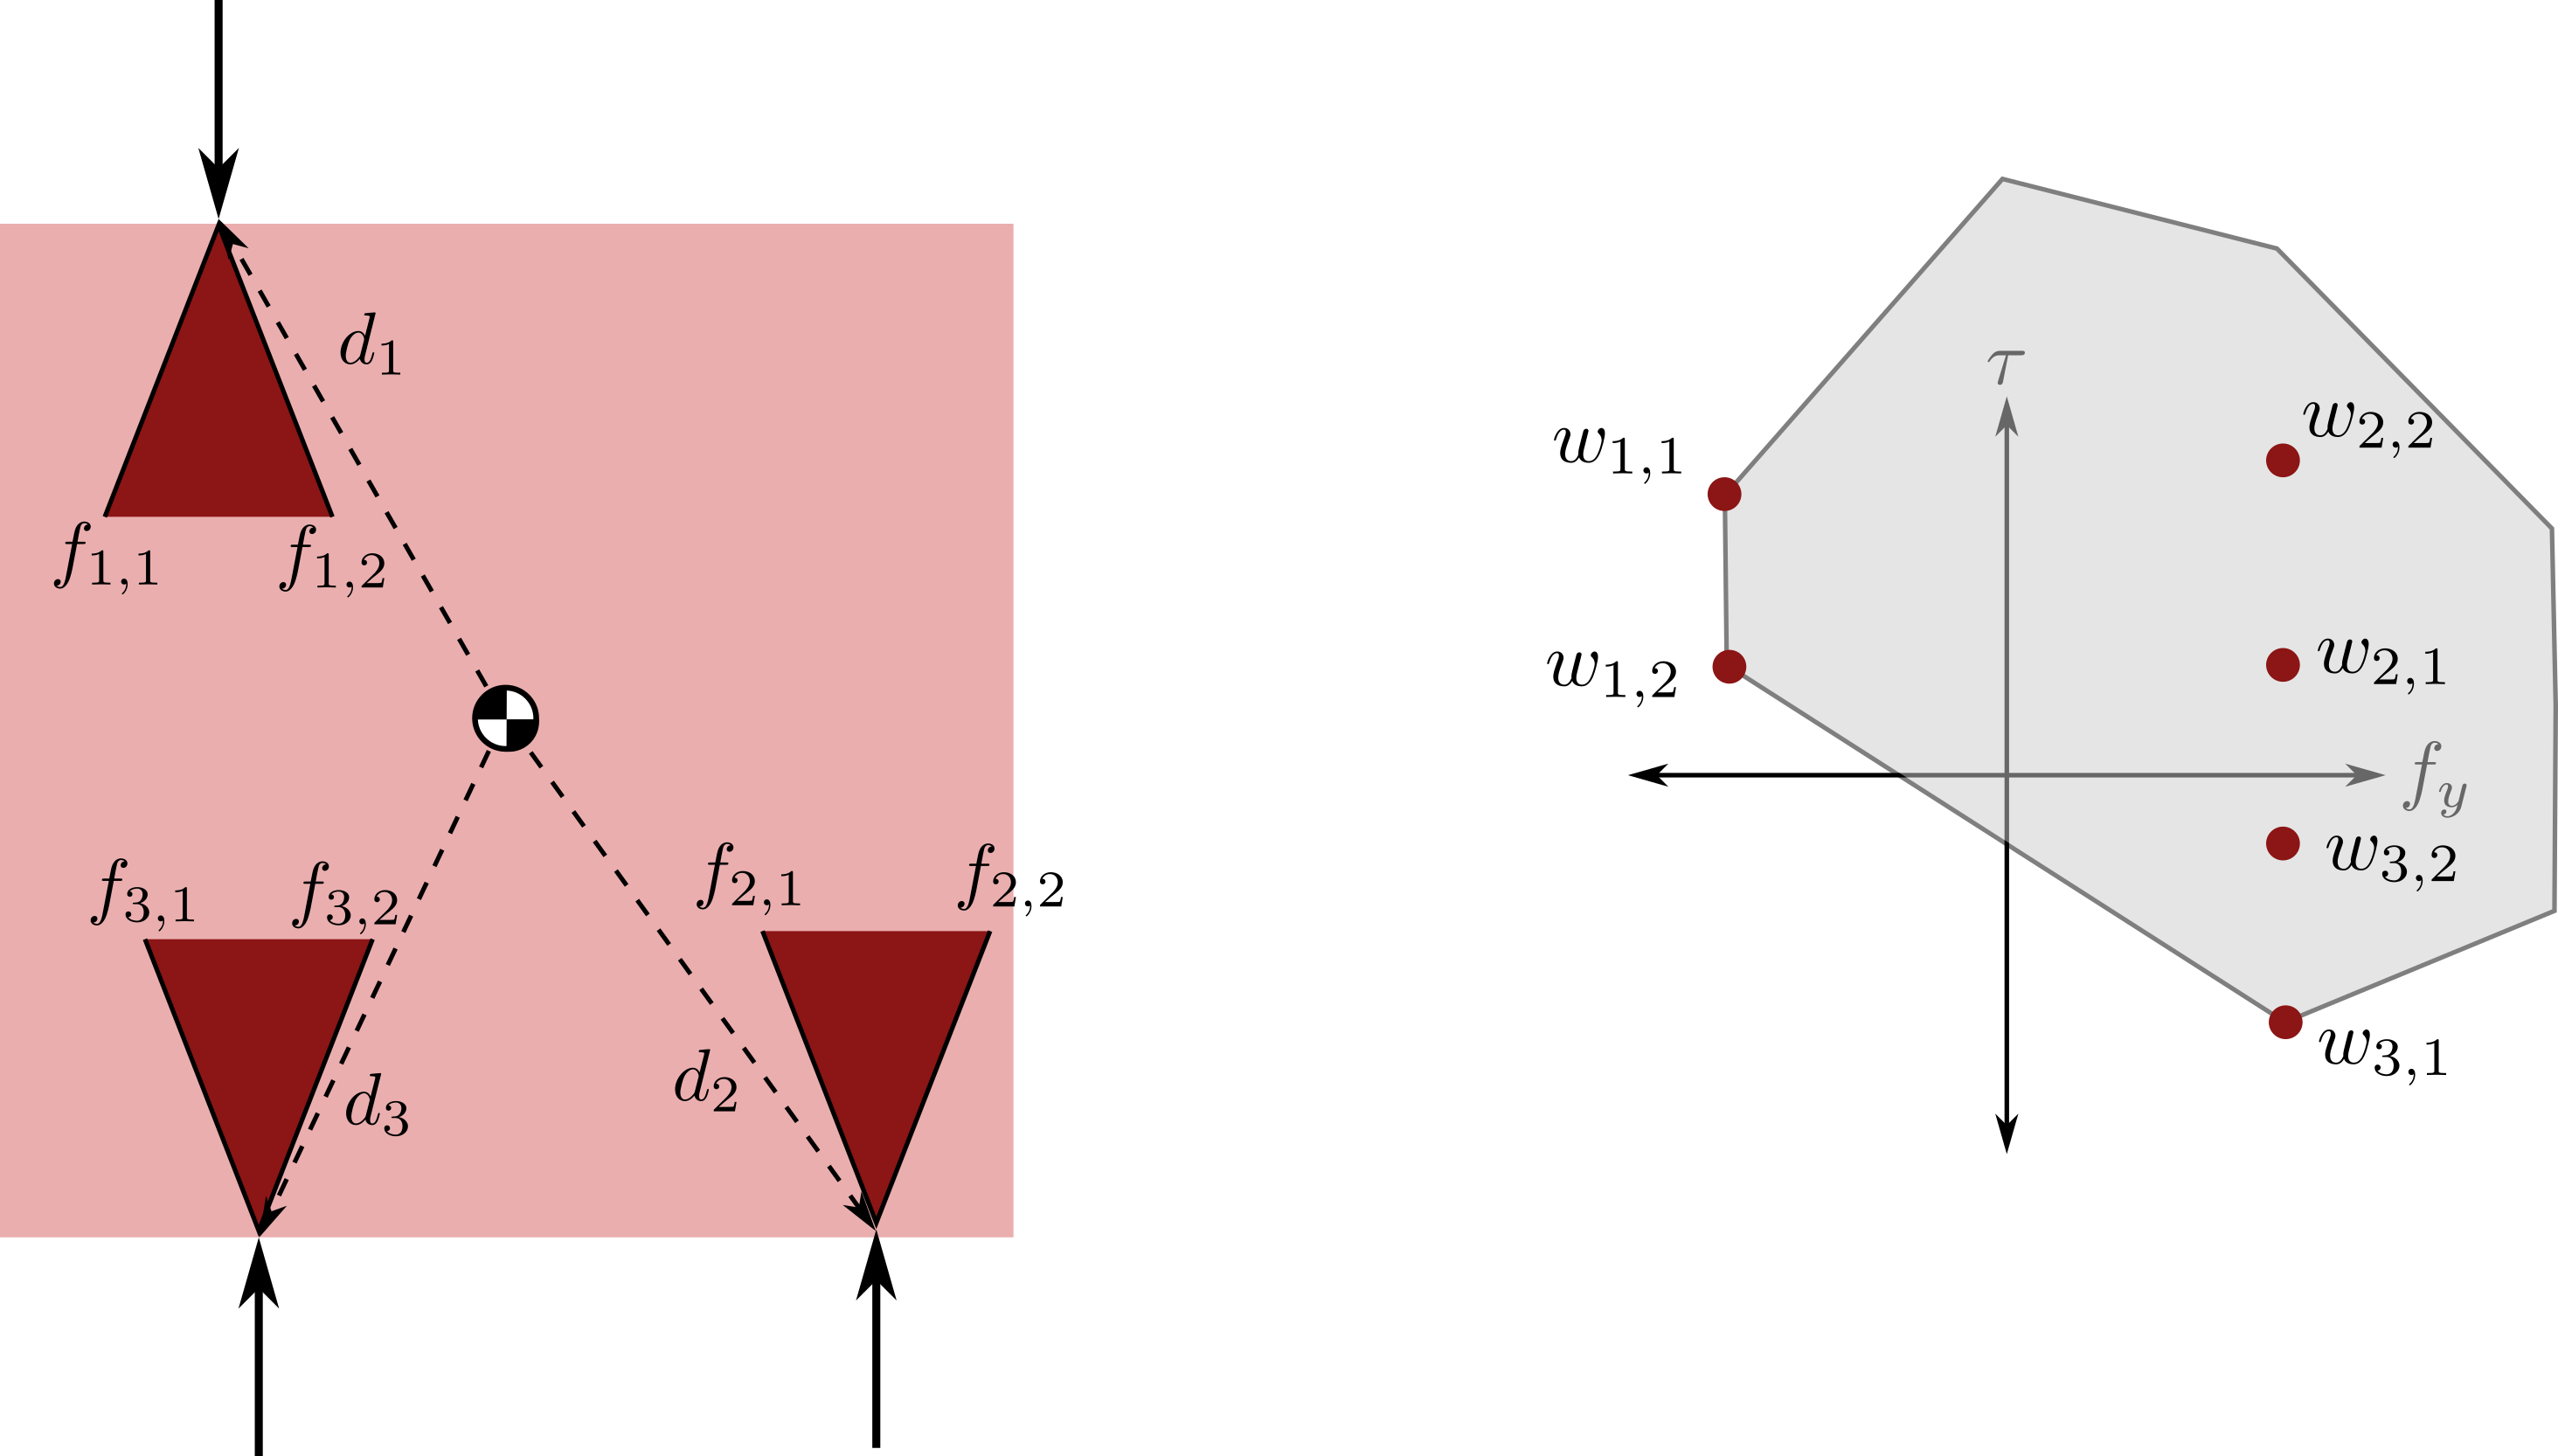
\includegraphics[width=0.75\textwidth]{tex/figs/ch26_figs/2Dexample_b.png}
\caption{A 2D grasp consisting of three point contacts with friction. The friction cones shown in the figure on the left yield the grasp wrench space in the figure on the right (showing only the vertical force and torque dimensions and assuming bounded contact force magnitudes). This grasp is in force closure because it can resist any external wrench (the origin is contained in the interior of $\mathcal{W}$).}
\label{fig:2dgrasp_b}
\end{center}
\end{figure}

\end{example}

\begin{example}[3D Object]
For 3D objects the grasp wrench space is in 6D (i.e. $\mathcal{W} \subseteq \R^6$). Theorem \ref{thm:vectorclosure}'s conditions therefore require that the grasp to be able to generate at least $7$ different wrenches, with $6$ being linearly independent, and where:
\begin{equation*}
  \sum_{k=1}^7 \beta_k \w_k = 0, \quad \beta_k > 0.
\end{equation*}
If frictionless contacts are assumed these conditions require \textit{at least} $7$ contact points and in the friction case \textit{at least} $3$ contacts are required.
\end{example}

\subsubsection{Grasp Wrench Hull}
The grasp wrench space $\mathcal{W}$ defines the set of all possible wrenches that can be applied to an object by a grasp, but unfortunately computing this set can be quite cumbersome in practice. One alternative approach for characterizing a grasp is through the definition of the \textit{grasp wrench hull}, which can be efficiently computed. Given a set of linearized friction cones $\mathcal{F}_i$ defined by the set of bounded forces $\{\f_{i,1}, \f_{i,2}, \dots, \f_{i,m}\}$ for each contact in the grasp, the wrench hull $\tilde{\mathcal{W}}$ is mathematically defined as:
\begin{equation*}
\begin{split}
\tilde{\mathcal{W}} = \{\w \mid \w = \sum_{i=1}^k \sum_{j=1}^m \alpha_{i,j}\w_{i,j}, \quad \w_{i,j} = \begin{bmatrix}
    \f_{i,j} \\ \lambda(\bd_i \times \f_{i,j})
    \end{bmatrix}, \quad \sum_{i=1}^k\sum_{j=1}^m \alpha_{i,j} = 1, \quad \alpha_{i,j} \geq 0\},
\end{split}
\end{equation*}
where $\bd_i$ is again the vector from the object center of mass to contact point $i$. Note that this is almost identical to the grasp wrench space definition except that the constraint $\sum_{j=1}^m \alpha_{i,j} \leq 1$ for all $i$ has been replaced by the constraint $\sum_{i=1}^k\sum_{j=1}^m \alpha_{i,j} = 1$. Put simply, the wrench hull is the convex hull of the wrenches $\w_{i,j}$! The difference between the grasp wrench space and the wrench hull is shown in Figure \ref{fig:wrenchhull} for the grasp from Example \ref{ex:2dobject}.
\begin{marginfigure} 
\begin{center}
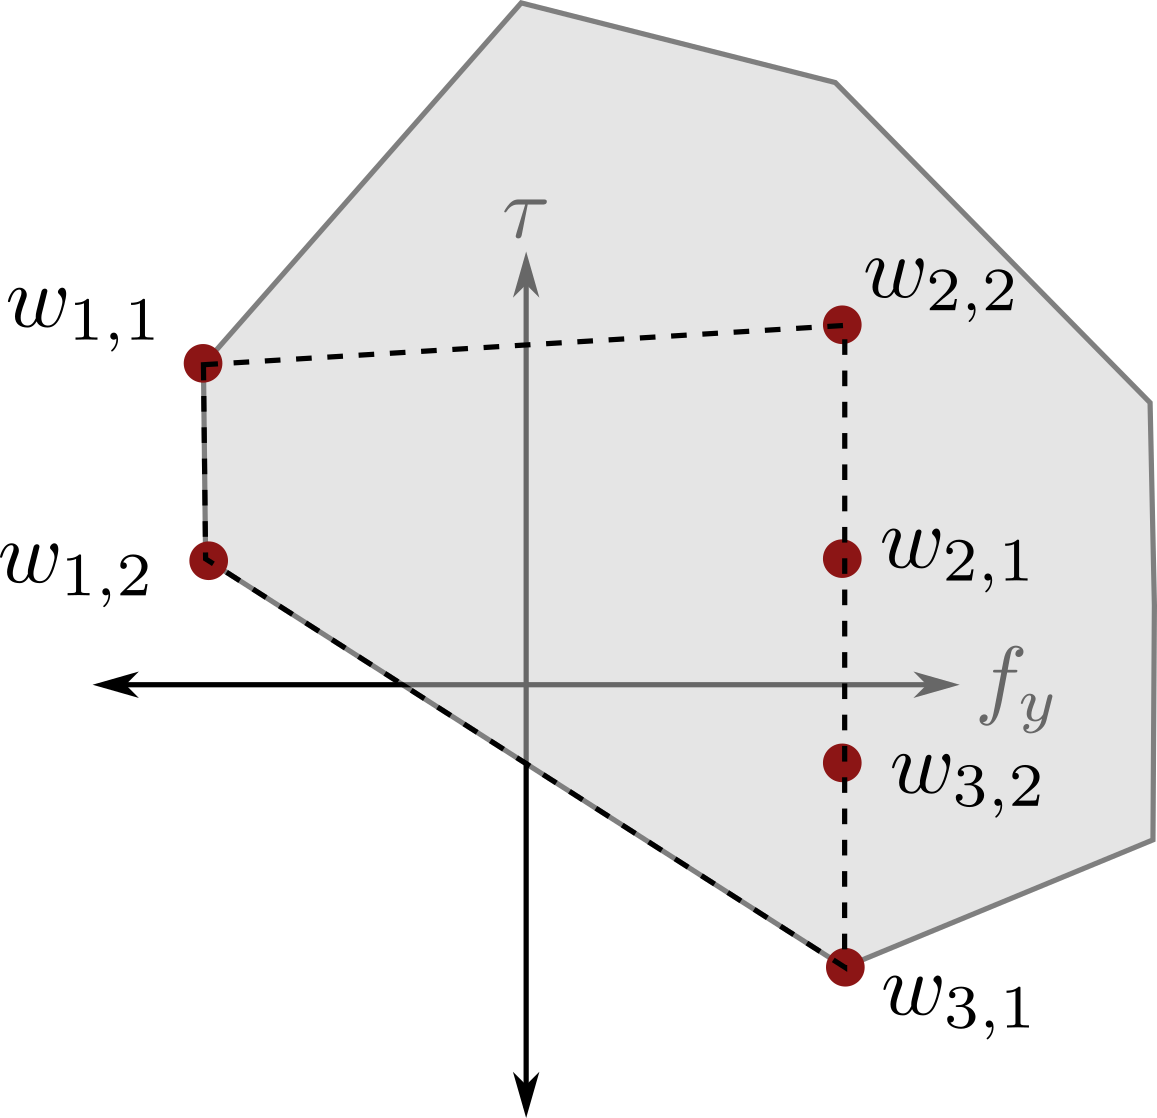
\includegraphics[width=0.8\textwidth]{tex/figs/ch26_figs/2Dexample_e.png}
\caption{Difference between grasp wrench space $\mathcal{W}$ (grey area) and wrench hull $\tilde{\mathcal{W}}$ (area enclosed by black dashed line) for the grasp in Example \ref{ex:2dobject}.}
\label{fig:wrenchhull}
\end{center}
\end{marginfigure}

Importantly the property $\tilde{\mathcal{W}} \subseteq \mathcal{W}$ holds by definition. Therefore grasp force closure is also guaranteed when the origin is in the interior of the wrench hull space. This fact, coupled with the fact that $\tilde{\mathcal{W}}$ is easier to compute than $\mathcal{W}$, makes it a useful characterization of grasps for evaluating grasp quality.

\subsubsection{Grasp Quality}
If the gripper could apply contact forces with infinite magnitude then a ``good'' grasp could simply be defined as one that is in force closure. However a more practical definition of grasp quality should be based on the assumption that the magnitude of the contact forces is bounded. In other words, a metric for grasp quality should quantify \textit{how well the grasp can resist external wrenches for a given bound on the contact force}.

To accomplish this, grasp quality metrics can be defined based on the definition of the grasp wrench hull $\tilde{\mathcal{W}}$. In particular, a useful metric is the radius of the largest ball centered at the origin that is completely contained in the grasp wrench hull (Figure \ref{fig:graspmetric}). This metric is useful for the following reasons:
\begin{enumerate}
    \item If the radius is zero, the origin is not contained in the interior of the wrench hull and therefore the grasp is not in force closure.
    \item For a radius greater than zero, the metric represents the magnitude of the \textit{smallest} external wrench that pushes the grasp to the limits. The direction from the origin to where the ball touches the boundary of $\mathcal{W}$ identifies the (opposite) direction in which the grasp is least able to resist external wrenches.
\end{enumerate}
\begin{marginfigure}[-12\baselineskip]
\begin{center}
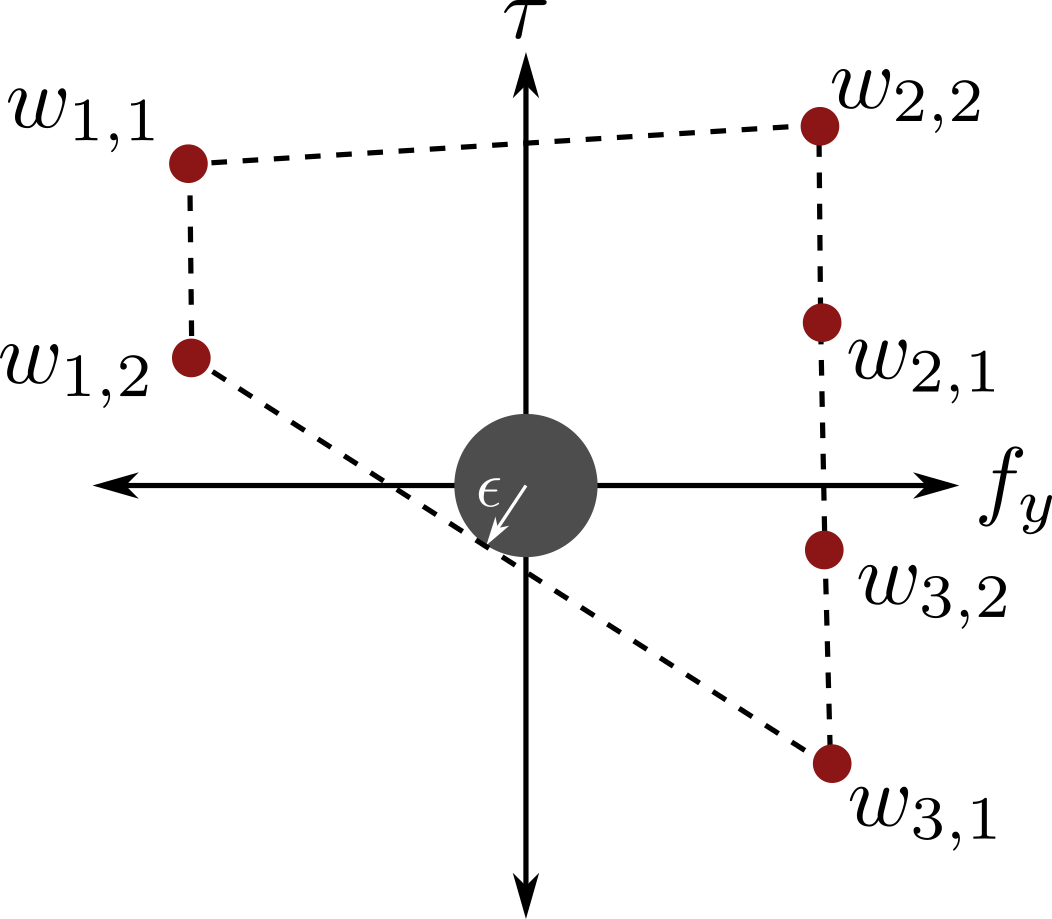
\includegraphics[width=0.8\textwidth]{tex/figs/ch26_figs/2Dexample_c.png}
\caption{Grasp quality can be measured as the radius $\epsilon$ of the largest ball contained in the grasp wrench hull centered at the origin.}
\label{fig:graspmetric}
\end{center}
\end{marginfigure}

Another method for quantifying the grasp quality is to compute the volume of the grasp wrench hull $\tilde{\mathcal{W}}$. This approach provides more of an average-case metric rather than a worst-case metric, and can help differentiate between different grasp spaces that have the same worst-case metric. For example Figure \ref{fig:graspmetric2} shows a grasp with the same worst-case metric as the grasp in Figure \ref{fig:graspmetric}, but which would be considered worse with respect to the volumetric (average-case) metric.
\begin{marginfigure} 
\begin{center}
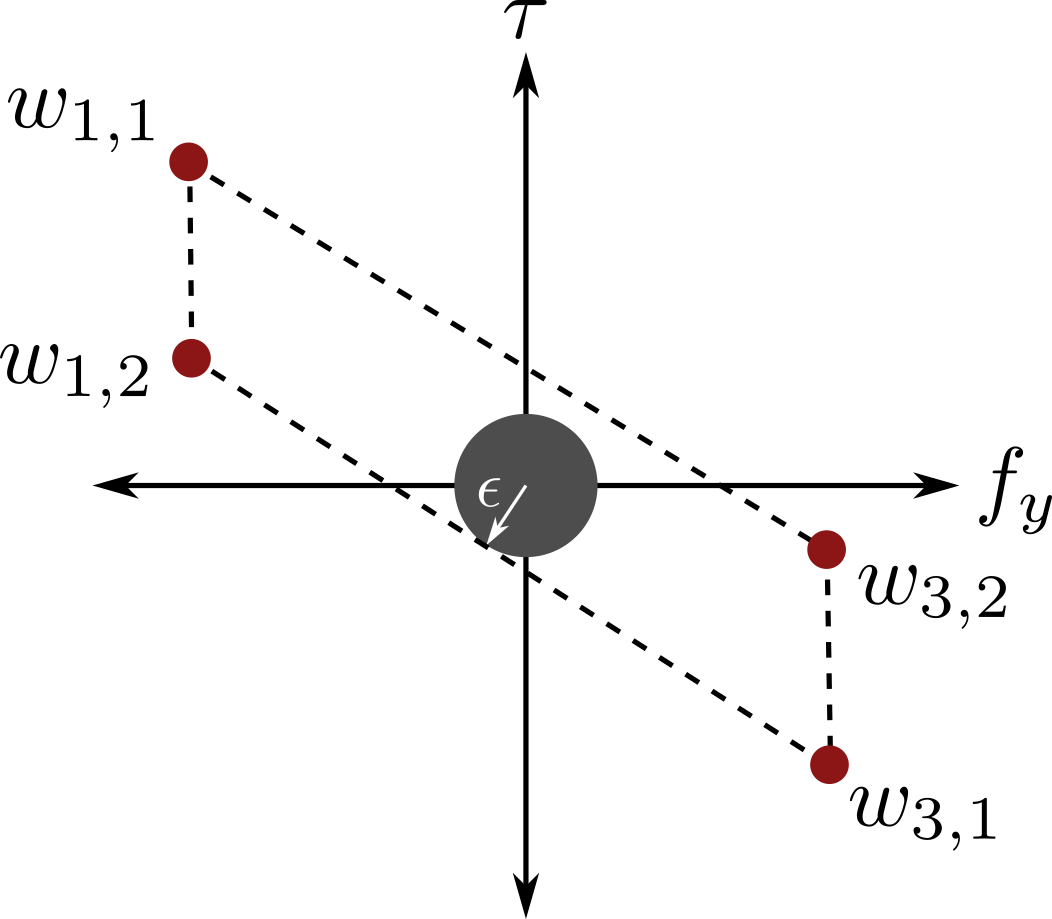
\includegraphics[width=0.8\textwidth]{tex/figs/ch26_figs/2Dexample_d.png}
\caption{Using the volume of $\tilde{\mathcal{W}}$ as a metric for grasp quality can help differentiate between two grasps with the same worst-case performance. For example this grasp would be considered less robust than the grasp in Figure \ref{fig:graspmetric} since it has smaller volume.}
\label{fig:graspmetric2}
\end{center}
\end{marginfigure}

\subsection{Grasp Force Optimization}
Recall from Section \ref{subsec:graspmodel} that for a particular contact model a grasp map matrix $G$ can be defined such that:
\begin{equation} \label{eq:f2w}
    \w = G\begin{bmatrix} 
    \f_1 \\ \vdots \\ \f_k
    \end{bmatrix},
\end{equation}
where $\f_i$ is the force vector associated with contact point $i$ and $\w$ is the total wrench applied to the object. Additionally, recall that the matrix $G$ also includes a rotational transformation such that the force vectors $\f_i$ are in local contact reference frames but $\w$ is represented in a common frame fixed in the object body (at the center of mass).

The next logical question to ask is how to compute force vectors $\{\f_i\}_{i=1}^k$ to achieve a desired wrench $\w$\footnote{The desired wrench may be used to counter an external disturbance (to maintain equilibrium) or to \textit{manipulate} the object.}. While one naive approach would be to just solve \eqref{eq:f2w} using a least-squares method, this would fail to account for any constraints on the force vectors. In particular, this section will focus on the point contact with friction model where each force vector $\f_i = [f^{(i)}_x,\: f^{(i)}_y,\: f^{(i)}_z]^\top $ must satisfy the friction cone constraint:
\begin{equation*}
\sqrt{{f^{(i)}_x}^2 + {f^{(i)}_y}^2} \leq \mu_{s,i} f^{(i)}_z, \quad f^{(i)}_z \geq 0,
\end{equation*}
where $\mu_{s,i}$ is the static friction coefficient for contact $i$. In this section the compact notation:
\begin{equation*}
\f_i \in \mathcal{F}_i, \quad \mathcal{F}_i \coloneqq \{\f \in \R^3 \mid \sqrt{f_x^2 + f_y^2} \leq \mu_{s,i} f_z, \quad f_z \geq 0\},
\end{equation*}
for the friction cone constraint will again be used.
It might also be desirable to include additional constraints on the force vectors, for example to account for hardware limitations (e.g. torque limits) or kinematic constraints. These additional constraints will be generally referred to by a convex constraint set $C$, such that $\f_i \in C$ is required for all $i = 1,\dots,k$. 

To summarize, the problem is to find a set of force vectors $\{\f_i\}_{i=1}^k$ such that \eqref{eq:f2w} is satisfied\footnote[][-3\baselineskip]{In the case that the desired wrench is used to counter an external disturbance, the condition \eqref{eq:f2w} is referred to as the equilibrium constraint.} and such that $\f_i \in \mathcal{F}_i$ and $\f_i \in C$ for $i = 1,\dots,k$. This problem can then be solved by formulating it as a convex optimization problem\cite{BoydWegbreit2007}\footnote{The problem is technically a second-order cone program because of the friction cone constraints.}:
\begin{equation} \label{eq:contactopt}
\begin{split}
\underset{\f_i, \:\: i \in \{1, \dots, k\}}{\text{minimize}} \:\: & J(\f_1, \dots, \f_k),\\
\text{s.t.} \:\:& \f_i \in \mathcal{F}_i, \quad i = 1,\dots,k, \\
&\f_i \in C, \quad i = 1,\dots,k, \\
&\w - G\begin{bmatrix} 
    \f_1 & \dots & \f_k
    \end{bmatrix}^\top  = 0,
\end{split}
\end{equation}
where $J(\cdot)$ is the objective function that is convex in each $\f_i$. Simply choosing $J = 0$ would result in a convex feasibility problem, but a more common choice is:
\begin{equation*}
J(\f_1, \dots, \f_k) = \max \{\lVert \f_1 \rVert, \dots, \lVert \f_k \rVert\},
\end{equation*}
which is the maximum applied force magnitude among all contact points.

Note that the fundamental disadvantage of this optimization-based approach is that the positions of all contacts with respect to the object's center of mass and the object's friction coefficients are assumed to be known. It is also assumed that the desired wrench $\w$ is known!


\subsection{Learning-Based Approaches to Grasping} \label{subsec:grasplearning}
Model-based methods for grasp evaluation and optimization require several assumptions that may be either difficult to validate in practice, or may not even be valid in all scenarios. These assumptions include:
\begin{enumerate}
    \item A coulomb (static) friction model defines the friction cone, and the coefficient $\mu_s$ is known.
    \item The object's geometry and mass distribution is known\footnote{One option would be to build a database of known objects, but this may not be scalable to real world problems.}, such that given a contact point the vector $\bd_i$ from the object's center of mass to the contact is known.
    \item The object is a rigid body.
    \item The desired forces $\f_i$ can be applied perfectly.
\end{enumerate}
Learning-based methods for grasp analysis\cite{BohgMoralesEtAl2014} can leverage data to decrease reliance on these assumptions, for example by not requiring explicit knowledge of the object's physical parameters. Learning-based methods can also combine the task of grasping with other parts of the manipulation pipeline, such as perception and motion planning. 

This section will introduce some recent learning-based approaches to robotic grasping, which is still a very active area of research. Specifically, these examples will demonstrate several learning-based strategies including approaches that create synthetic training data from model-based simulators and approaches that use real hardware to generate data.

\subsubsection{Choosing a Grasp Point from an RGB Image\cite{SaxenaDriemeyerEtAl2008}}
The objective of this supervised learning approach was to learn how to find a good grasp point in an RGB image of an object, and then generate a prediction of the point's 3D position. Since supervised learning techniques can require a lot of training data, this approach auto-generated training images \textit{synthetically} using realistic rendering techniques (see Figure \ref{fig:saxenacup}). The use of synthetic data also made it easier to collect a diverse training set including images with different lighting, object color, and object orientation and size.
\begin{marginfigure} [3\baselineskip]
\begin{center}
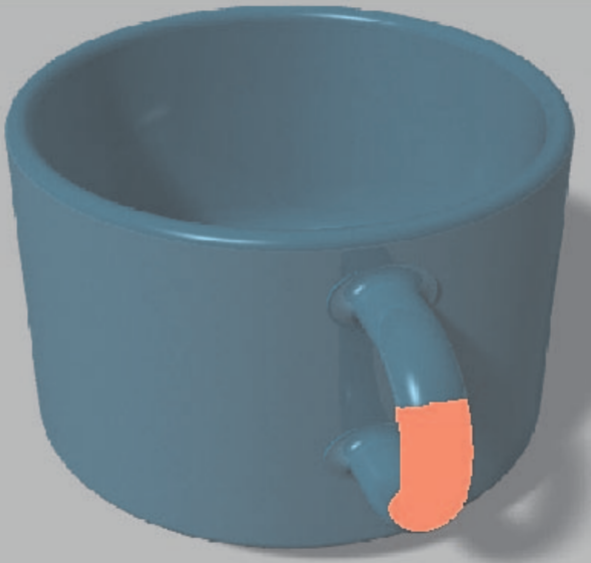
\includegraphics[width=0.6\textwidth]{tex/figs/ch26_figs/saxenacup.png}
\caption{Synthetic image of a cup and its labeled grasp point from Saxena et al. (2008).}
\label{fig:saxenacup}
\end{center}
\end{marginfigure}
Once a model was trained to produce good grasp point classifications, 3D predictions of the target grasp position were generated by \textit{structure-from-motion}, where two images were used to triangulate the point in space. While there are certainly limitations to this approach, this work produced promising results, including good grasp success rates on novel objects (that weren't included in the training dataset). This work also had substantial influence on future learning-based grasping and manipulation approaches.

\subsubsection{Exploiting Simulation and a Database of Objects to Predict Grasp Success\cite{MahlerPokornyEtAl2016}}
The Dex-Net approach for learning to grasp is another supervised learning approach that relies on simulations to generate training data. Specifically this approach assumes a parallel jaw gripper and contains a large ($>10,000$) database of 3D object models.
For each model in the Dex-Net database, the simulator uses analytical (model-based) techniques to evaluate a large number of potential grasps for probability of success\footnote{The Dex-Net database consists of $2.5$ million tested grasps.}. This is accomplished by empirically sampling a grasp some number of times and determining (through simulation) the percentage that result in force closure\footnote{There is simulated uncertainty in object and gripper pose, as well as the surface friction.}. The database of objects and potential grasps can then be used to train a model to predict the probability of force closure for a new grasp/object.

In practice a number of candidate grasps are generated for a given (potentially novel) object, are evaluated by the learned model to predict probability of success, and then a \textit{multi-armed bandit}\footnote[][-2\baselineskip]{A fundamental reinforcement learning problem focused on uncertain decision making.} approach is used to select which grasp to take. The learned models are then updated based on the outcome of the action for continuous improvement. This work showed that leveraging the prior information from the object database can significantly improve grasping for new objects (even if they are not in the database), and later improvements have enhanced the approach even further.
\begin{marginfigure}
\begin{center}
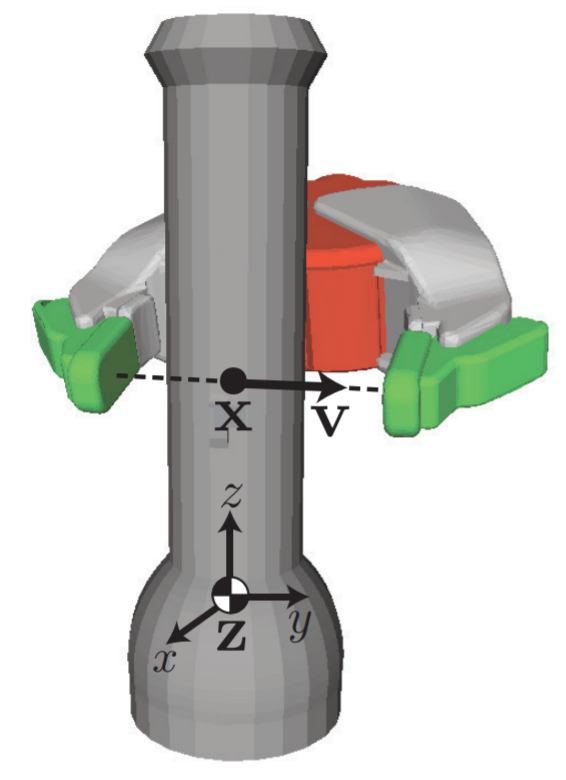
\includegraphics[width=0.5\textwidth]{tex/figs/ch26_figs/dexnet.png}
\caption{Dex-Net grasps are parameterized by the centroidal position of the gripper $x$ and the approach direction $v$, Mahler et al. (2016).}
\label{fig:dexnet}
\end{center}
\end{marginfigure}

\subsubsection{Learning to Grasp Through Real-World Trial-and-Error\cite{LevinePastorEtAl2018}}
Instead of leveraging simulators to generate synthetic data this work uses hardware experiments to generate real-world data. The resulting experiences are then used in a self-supervised approach to learn an \textit{end-to-end} framework to grasp objects in cluttered environments. One of the reasons this work is significant is the lack of assumptions that are made: 3D object models are not needed, only RGB images are required, it does not use contact models or simulated data, no physical object information is used, and no hand-engineered path/grasp planning algorithms are used.
Instead the system just learns through trial-and-error, exploring approaches to actuate the robot arm and gripper that eventually lead to robust grasps.

This approach showed impressive results over hand-designed or open-loop approaches, but at the cost that it took six months and a large number of robots to generate enough training data.

\subsection{Learning-Based Approaches to Manipulation} \label{subsec:manipulationlearning}
The previous sections of this chapter have focused on the problem of grasping, but many robotic manipulation tasks involve more than simply grasping an object. For example it is possible to manipulate objects \textit{without} force closure grasps, such as by pushing the object\footnote{Not only is it possible, but may be necessary if the object is too large or heavy to grasp.}. Many manipulation tasks that do involve grasping also involve other complex steps, such as using the grasped object to manipulate other objects (e.g. hitting a hammer with a nail) or placing the object in a certain position (e.g. inserting a key into a lock). This section will introduce at a high-level some interesting and foundational problems in manipulation, and present the high-level ideas found in some recent research on learning-based approaches to solving them.

\subsubsection{Planar Pushing}
Planar pushing is a fundamental manipulation task where the goal is to control the pose of an object in a 2D setting by only using ``pushing'' contacts. While the contact point models used for grasping can also be applied in this problem, the interaction of the object and the surface must also be accounted for. 

Similar to the physics-based contact models for grasping, physics-based models can also be developed to predict the sliding interactions between the object and the surface. In particular, the concept of a \textit{friction limit surface}\cite{KaoLynchBurdick2016} can be used to model the interaction between the object and the surface. The friction limit surface is a boundary in wrench space that separates wrenches that the surface can apply to the object through friction and those it can't. The part of the wrench space enclosed by this surface will contain the origin (i.e. the zero wrench), and most importantly whenever the object is \textit{slipping} the wrench applied on the object lies \textit{on the friction limit surface}. This surface can be determined numerically if the coefficient of friction, the contact area, and the pressure distribution are known. For simplicity, it is common to approximate this surface as an ellipsoid. To summarize:
\begin{enumerate}
    \item If an external wrench applied to the object is within the region of the wrench space enclosed by the friction limit surface, friction between the object and the surface will cause the object to remain motionless.
    \item If the part slides quasistatically\footnote{Assumption that the part moves slowly enough that inertial effects are negligible.}, the pushing wrench must lie on the friction limit surface and the motion (velocity) of the object can be determined.
\end{enumerate}

The friction limit surface provides the foundation for a physics-based model that predicts how an object will slide across a surface under external contact forces. Such a model could be used to design a controller (e.g. with model predictive control) for planar pushing tasks. However, these physics-based models are based on approximations and assumptions\marginnote{Assumptions in physics-based pushing model: ellipsoidal friction limit surface, coulomb friction, perfectly planar object/surface, rigid body object, physical properties of object are known.} that may impact their accuracy or applicability to real problems. In fact some studies have been performed to evaluate the accuracy of physics-based pushing models\cite{YuBauzaEtAl2016}.

While physics-based controllers such as model predictive control can handle some uncertainty via feedback control mechanisms, it is still desirable to improve the modeling accuracy and eliminate assumptions requiring knowledge of the parameters that define the models\footnote{For example the physical properties of the object and surface.}. Learning-based approaches are one possible solution to some of these challenges, where real-world data can be used to either completely replace or augment the physics-based models.

In fact, recent work\cite{KlossSchaalEtAl2020} has compared the use of physics-based, hybrid (physics + learning), and learning-based models for planar pushing tasks. In this work the hybrid model learned a mapping from sensor measurements (RGB images) into a set of parameters that were required for the physics-based motion model and the learning-based model just directly learned a single neural network for mapping sensor measurements to motion predictions directly. As might be expected the hybrid approach achieved better generalization by leveraging the physics-based model's structure, while the learning-based approach overfit to the training data\footnote{This is a classic example of bias-variance tradeoff in modeling.}.


\subsubsection{Contact-Rich Manipulation Tasks}
Many 6D manipulation problems involve grasping an object and then using it to physically interact with the environment. Classic everyday examples include hitting a nail with a hammer, inserting a key into a lock, and plugging a cord into an electrical outlet. These types of \textit{contact-rich} tasks tasks typically rely on multiple different sensing modalities including haptic and visual feedback. Consider the task of inserting a key into a lock: without sight it would be challenging to correctly position the key and without tactile sensing (e.g. force/torque sensing) it would be challenging to know when the key is perfectly aligned and can be inserted.

However, it can be quite challenging to \textit{integrate} multiple sensing modalities toward a common task, especially when the sensing modalities are so different and since manipulation tasks can be quite complex. One approach may be to individually develop systems for different subtasks and manually find a common interface to stitch them together, however this could be challenging from a system engineering perspective. An alternative is to use machine learning techniques to automatically integrate the sensing modalities.

One learning-based approach to this problem is to design an end-to-end system that takes as input all sensor data streams and outputs actions for the robot to execute the task. However, when implemented in a naive way (e.g. a single massive neural network architecture) end-to-end approaches can be data inefficient. An alternative is to add additional structure to the learning-based approach by leveraging some insights into the problem, similar to how the physics-based motion model was used in the learning-based planar pushing example discussed in the previous section.

A structured approach for manipulation tasks relying on multiple sensing modalities is introduced by Lee et al.\cite{LeeZhuEtAl2019}. In this work an end-to-end system that takes sensor data streams as input and outputs robot actions is split into two parts: first transforming the multi-modal sensor data streams into a low-dimensional feature representation that contains task relevant information\footnote{This is accomplished by training an autoencoder network.}, and then using these features as the input to a learned policy that generates robot actions. In other words, the insight is that the learning process can be made more efficient by first learning a way to compress and summarize all of the sensor data, and then learning how to use the summarized information to generate a good policy. Another benefit to this approach is that the sensor data \textit{encoder} can generalize more effectively to new tasks, meaning that only the policy portion needs to be retrained!
